\documentclass[11pt]{article}

\usepackage[margin=1in]{geometry}
\usepackage{xcolor}
\usepackage{graphicx}
\usepackage{booktabs}
\usepackage{amsmath}
\usepackage{enumitem}
\usepackage{listings}
\usepackage[hidelinks]{hyperref}

\newcommand{\file}[1]{\texttt{\detokenize{#1}}}
\newcommand{\code}[1]{\texttt{\detokenize{#1}}}

\newsavebox{\gpbox}
\newenvironment{finding}[1]{%
  \begin{lrbox}{\gpbox}\begin{minipage}{0.94\linewidth}%
  \textbf{\textcolor{green!35!black}{#1}}\par\smallskip\small}%
 {\end{minipage}\end{lrbox}%
  \begin{center}\setlength{\fboxrule}{0.7pt}%
  \fcolorbox{green!35!black}{green!5}{\usebox{\gpbox}}\end{center}}
\newenvironment{caveat}[1]{%
  \begin{lrbox}{\gpbox}\begin{minipage}{0.94\linewidth}%
  \textbf{\textcolor{red!55!black}{#1}}\par\smallskip\small}%
 {\end{minipage}\end{lrbox}%
  \begin{center}\setlength{\fboxrule}{0.7pt}%
  \fcolorbox{red!55!black}{red!4}{\usebox{\gpbox}}\end{center}}

\title{\vspace{-1.5em}Hydration-site clustering: old vs new\\[0.3em]
\large The same CRY1/AN139 trajectory analysed two ways}
\author{}
\date{}

\begin{document}
\maketitle
\vspace{-2.5em}

\section*{Summary}

The original GRAND clustering and the pipeline's \file{ev71_postprocess.py} were run on
\textbf{the identical 2500-frame trajectory}, with the same sphere, cutoff and frame
sampling. Only the analysis differs, so any difference is method, not sampling.

\textbf{They agree on every persistent hydration site.} Above an occupancy of 0.4 the two
site sets are identical. Where they overlap, sites coincide to \textbf{0.36 \AA{}}.

\textbf{The old method reports 302 clusters, the new one 176.} The 126-cluster difference is
almost entirely one-frame noise: the extra clusters have median occupancy \textbf{0.00}.
This is the ghost-exclusion fix removing spurious water observations, and it matters because
those clusters are what depressed the precision and Tanimoto figures in the original study.

\section{Setup}

\begin{center}\small
\begin{tabular}{@{}l l@{}}
\toprule
Trajectory & \file{GCMC_Grand/CRY1AN139-raw.dcd}, 2500 frames (complete production) \\
Old result & \file{CRY1AN139-lig-clusts.pdb}, already present, from GRAND \code{cluster_waters} \\
New result & \file{ev71_postprocess.py}, \code{--cluster-stride 1} (full parity) \\
Common settings & 10 \AA{} sphere on the ligand, 2.4 \AA{} average-linkage cutoff \\
\midrule
New-method cost & 71\,050 water observations, 20.2 GB distance matrix, 16 min \\
\bottomrule
\end{tabular}
\end{center}

The one substantive difference between the implementations is ghost handling. GRAND shifts
inactive ghost waters \emph{before} imaging, which can bring non-interacting molecules back
toward the ligand; the new script images first, shifts after, and additionally excludes
inactive ghosts frame by frame.

\section{Result 1 --- the site sets}

\begin{center}
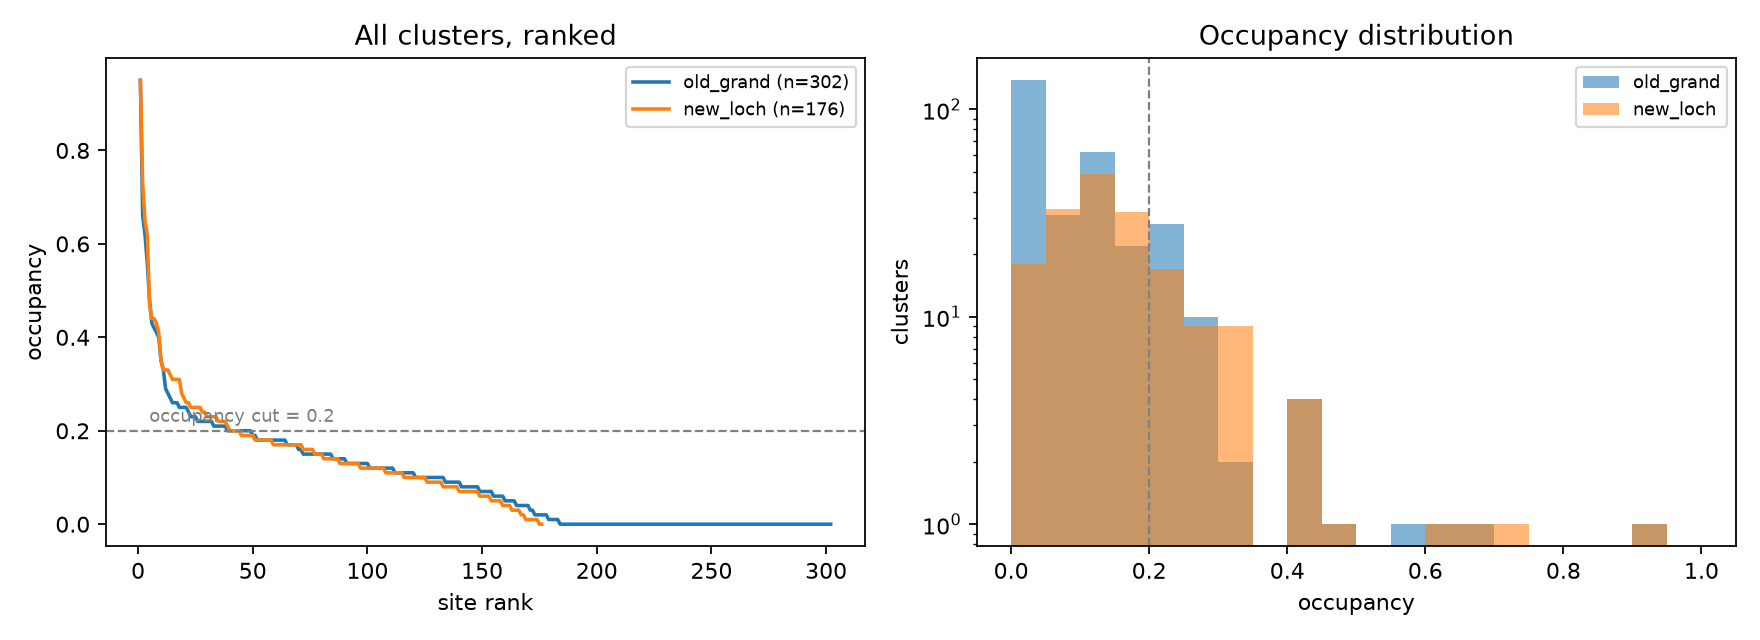
\includegraphics[width=0.98\linewidth]{figures/AN139method_occupancy.png}
\end{center}

Left: every cluster, ranked by occupancy. The two curves lie on top of one another for the
first $\sim$130 sites and then diverge --- the old method continues with a long tail of
clusters that the new one does not produce. Right: the same thing binned (note the log
scale); the excess is entirely in the lowest bin.

\begin{center}\small
\begin{tabular}{@{}l r r r@{}}
\toprule
& all clusters & occupancy $\ge 0.2$ & median occupancy of the extras \\
\midrule
old (GRAND) & 302 & 49 & \\
new (pipeline) & 176 & 44 & \\
\midrule
matched & 168 & 39 & \\
old only & 134 & & \textbf{0.00} \\
new only & 8 & & 0.08 \\
\bottomrule
\end{tabular}
\end{center}

The 134 old-only clusters have a median occupancy of \textbf{0.00} --- they are occupied in
about one frame out of 2500. They are not distant artifacts: their distance to the ligand
(median 3.8 \AA{}) is the same as the matched sites'. They are one-off water positions inside
the sphere that the ghost-exclusion step removes.

\section{Result 2 --- how well they agree}

\begin{center}
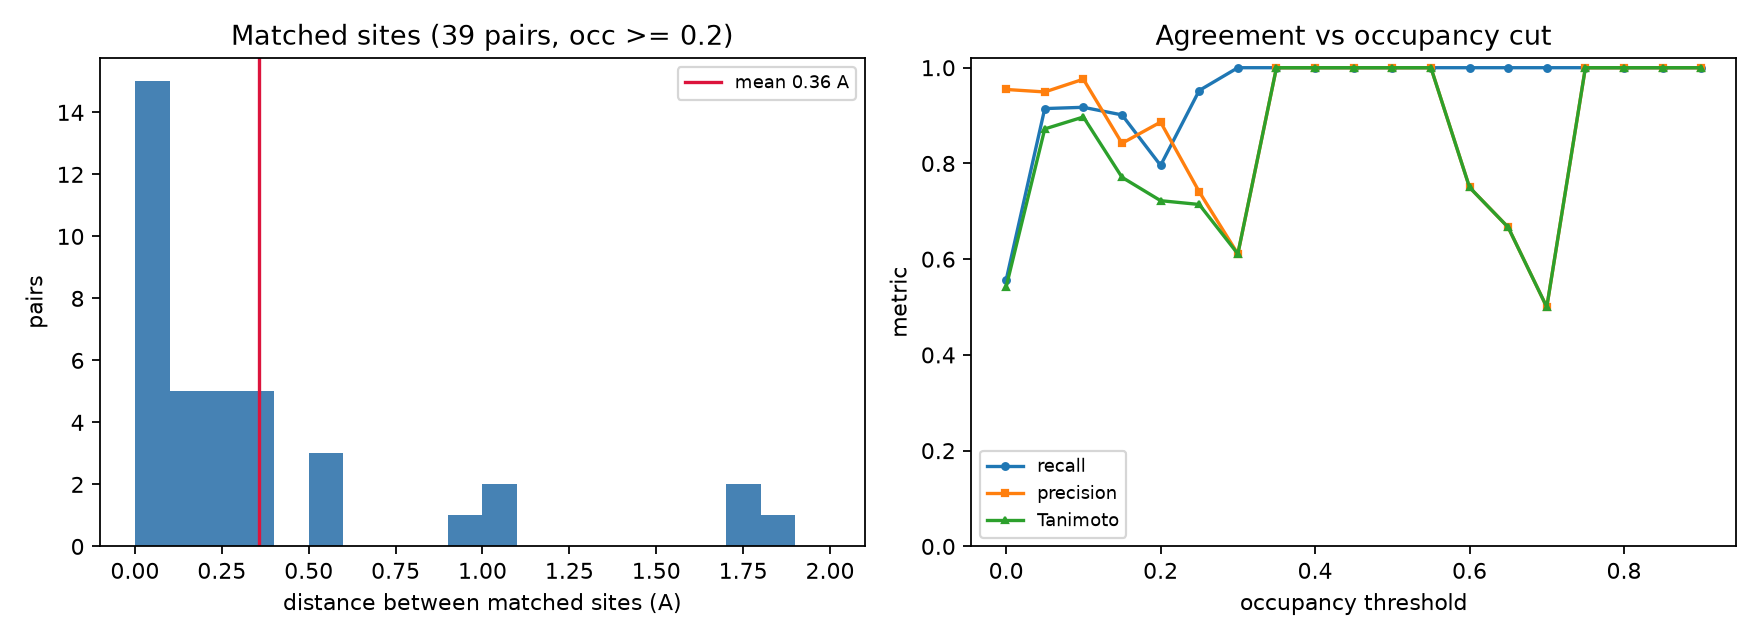
\includegraphics[width=0.98\linewidth]{figures/AN139method_agreement.png}
\end{center}

Left: the 39 matched persistent sites, mean separation \textbf{0.36 \AA{}}. For scale, two
independent GCMC \emph{simulations} of this system match at $\sim$1.1--1.3 \AA{}. Two
analyses of the \emph{same} trajectory should agree far better than that, and they do.

Right: sweeping the occupancy cut. This is the most informative panel.

\begin{center}\small
\begin{tabular}{@{}r r r r r r r@{}}
\toprule
cut & $n_{\text{old}}$ & $n_{\text{new}}$ & matched & recall & precision & Tanimoto \\
\midrule
0.00 & 302 & 176 & 168 & 0.556 & 0.955 & 0.542 \\
0.10 & 133 & 125 & 122 & 0.917 & 0.976 & 0.897 \\
0.20 & 49 & 44 & 39 & 0.796 & 0.886 & 0.722 \\
0.30 & 11 & 18 & 11 & 1.000 & 0.611 & 0.611 \\
\textbf{0.40} & \textbf{9} & \textbf{9} & \textbf{9} & \textbf{1.000} & \textbf{1.000} & \textbf{1.000} \\
0.50 & 4 & 4 & 4 & 1.000 & 1.000 & 1.000 \\
\bottomrule
\end{tabular}
\end{center}

\begin{finding}{Two things to take from this table}
\textbf{Precision is 0.955 even with no occupancy cut.} Almost every site the new method
reports is also in the old set. The new method is not finding different water --- it is
declining to report spurious clusters. The disagreement is one-directional.

\textbf{Above a 0.4 cut the sets are identical.} Every persistent hydration site, the kind
that actually gets reported, is found by both. The entire discrepancy lives in clusters that
appear in a handful of frames.
\end{finding}

\section{Result 3 --- where the disagreement sits}

\begin{center}
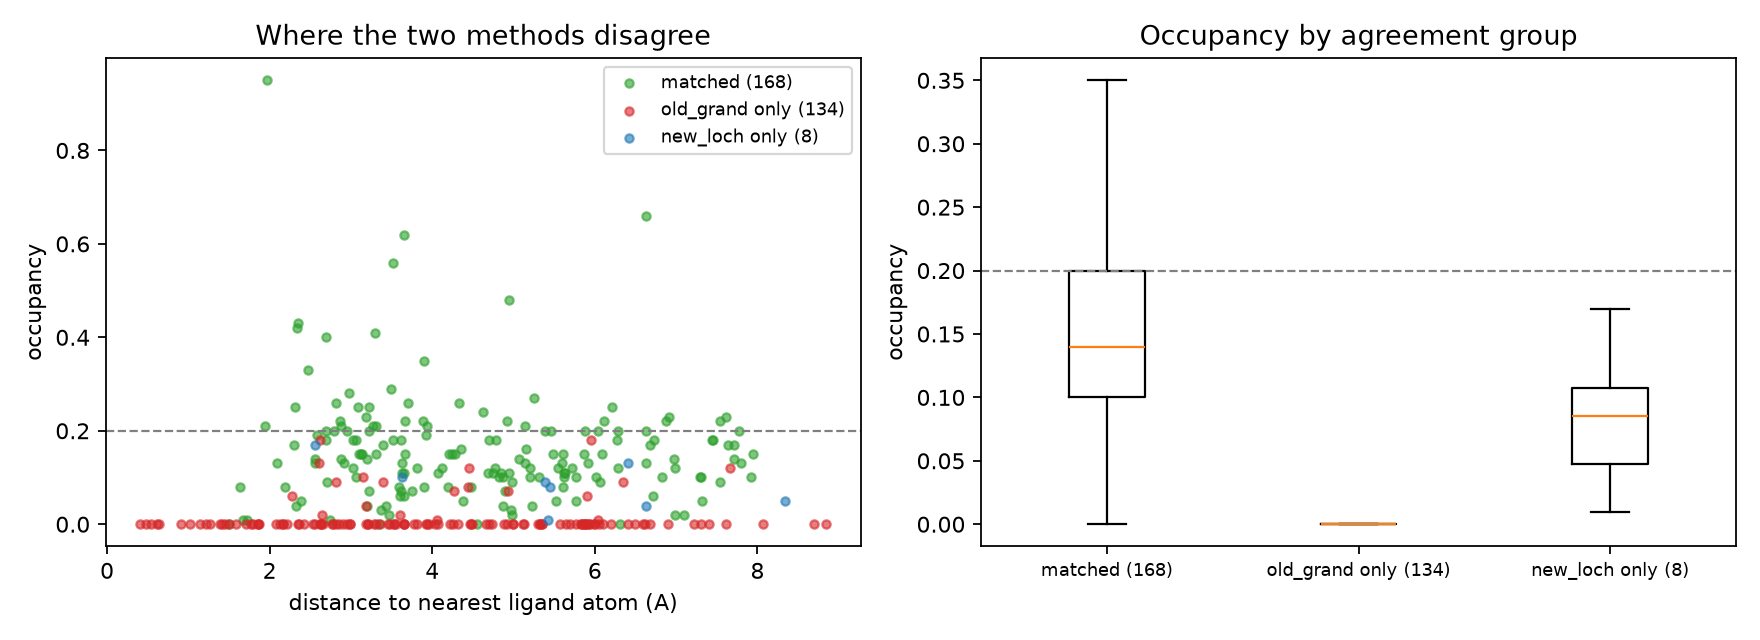
\includegraphics[width=0.98\linewidth]{figures/AN139method_disagreement.png}
\end{center}

Every old-only cluster (red) sits at the bottom of the occupancy axis, spread across the same
range of ligand distances as the matched sites. There is no spatial signature --- these are
not, for instance, ghosts piled up next to the ligand. They are simply water seen once.

\section{Why this matters for the published numbers}

The original study reported, for AN139 against crystallographic waters, a recall of 0.870
against a precision of \textbf{0.211} and a Tanimoto of \textbf{0.205}, and explained the low
values as follows:

\begin{quote}\small
``besides matched clusters there are many additional unmatched clusters, resulting in a low
value of Precision and Tanimoto similarity coefficient. This observation is expected, as
crystallographic structures provide a static and ensemble-averaged representation of
hydration and may not resolve transient or weakly occupied water molecules.''
\end{quote}

That reasoning is sound as far as it goes, but this comparison shows a second contribution
the study could not have seen: of the 302 clusters, \textbf{134 are one-frame artifacts of
ghost handling}, not transient physical hydration. Recomputing those metrics on the cleaned
176-cluster set would raise precision and Tanimoto without changing recall.

\begin{caveat}{What this does \emph{not} show}
Only one system and one trajectory. And this compares two \emph{analyses}, not two
\emph{simulation engines} --- it says nothing about whether GRAND and Loch sample the same
water, only that given identical frames they identify the same sites. The engine comparison
needs matched-length production runs on the same system, which do not yet exist.
\end{caveat}

\section{Reproducing this}

\begin{lstlisting}[basicstyle=\ttfamily\footnotesize]
python ev71_postprocess.py \
  --topology  <GCMC_Grand>/CRY1AN139-ghosts.pdb \
  --trajectory <GCMC_Grand>/CRY1AN139-raw.dcd \
  --ghost-file <GCMC_Grand>/gcmc-ghost-wats.txt \
  --output-dir new --prefix AN139new \
  --sphere-radius 10.0 --cluster-cutoff 2.4 --cluster-stride 1 \
  --max-distance-memory-gb 64

python compare_water_sites.py \
  --sites old_grand <GCMC_Grand>/CRY1AN139-lig-clusts.pdb \
  --sites new_loch  new/AN139new-lig-clusts.pdb \
  --reference old_grand --plots \
  --ligand-reference <GCMC_Grand>/CRY1AN139-ghosts.pdb \
  --output-dir . --prefix AN139method
\end{lstlisting}

\noindent\small
\code{--cluster-stride 1} is needed for parity with GRAND and costs 20 GB and 16 minutes. A
stride of 5 gives the same persistent sites in 30 seconds and 0.6 GB; the stride is recorded
in the metrics JSON, so the approximation is never silent.

\end{document}
